\documentclass[12pt]{article}
\usepackage{amsfonts, epsfig}
\usepackage[authoryear]{natbib}
\usepackage{graphicx}
\usepackage{fancyhdr}
\pagestyle{fancy}
\lfoot{\texttt{comsm0034.github.io}}
\lhead{IP\&B - 2\_information\_in\_the\_brain - Conor}
\rhead{\thepage}
\cfoot{}
\begin{document}

\section*{Information in the brain} 

We will look at two applications of information theory to the study of
the brain; the first, dealt with here is calculating the information
content of spike trains. This is an example of data analysis for
interpreting experimental data in neuroscience. The second, infomax,
is an interpretation of information processing in the brain, which may
have something to tell us about how to compute with data; this will be
in the next chapter.

\subsection*{The information content of spike trains}

Neurons communicate using action potentials, discrete voltage spikes
that travel from neuron to neuron. This is the main way information
propagates through the brain. The action potentials, often also called
spikes, are stereotypical in amplitude, so the information that carry is
represented in their timing. Spike trains are very noisy, repeated
responses to the same stimulus tend to be very different; for example,
in Fig.~\ref{fig_zebra_finch} there are raster plots from neurons in
the auditory area of the zebra finch brain; a raster plot is a plot
with a little dash for each spike. The individual trials run
horizontally. As you can see there is considerable variation from
trial to trial. This variability is unsurprising, the brain is made up
of multiple interlocking ad hoc networks so there is likely to be
considerable background noise. The question is then, how much
information do spike trains carry.

\begin{figure}[htb]
\begin{center}
\begin{center}
\begin{tabular}{cl}
{\bf A}&\\&\hspace{0cm} 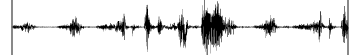
\includegraphics[width=6.55cm]{song.png}\\
{\bf B}&\\&
\setlength{\unitlength}{0.017pt}
\setlength{\fboxsep}{0pt}
\framebox{
\begin{picture}(9999,1240)(0,0)
\put(197,40){\line(0,1){80}}
\put(212,40){\line(0,1){80}}
\put(236,40){\line(0,1){80}}
\put(402,40){\line(0,1){80}}
\put(499,40){\line(0,1){80}}
\put(569,40){\line(0,1){80}}
\put(631,40){\line(0,1){80}}
\put(658,40){\line(0,1){80}}
\put(722,40){\line(0,1){80}}
\put(1406,40){\line(0,1){80}}
\put(1574,40){\line(0,1){80}}
\put(1658,40){\line(0,1){80}}
\put(1727,40){\line(0,1){80}}
\put(1924,40){\line(0,1){80}}
\put(2055,40){\line(0,1){80}}
\put(2131,40){\line(0,1){80}}
\put(2806,40){\line(0,1){80}}
\put(2861,40){\line(0,1){80}}
\put(2881,40){\line(0,1){80}}
\put(2909,40){\line(0,1){80}}
\put(3051,40){\line(0,1){80}}
\put(3277,40){\line(0,1){80}}
\put(3368,40){\line(0,1){80}}
\put(3662,40){\line(0,1){80}}
\put(4248,40){\line(0,1){80}}
\put(4851,40){\line(0,1){80}}
\put(4895,40){\line(0,1){80}}
\put(4914,40){\line(0,1){80}}
\put(5030,40){\line(0,1){80}}
\put(5134,40){\line(0,1){80}}
\put(5206,40){\line(0,1){80}}
\put(5272,40){\line(0,1){80}}
\put(5765,40){\line(0,1){80}}
\put(5796,40){\line(0,1){80}}
\put(5935,40){\line(0,1){80}}
\put(6094,40){\line(0,1){80}}
\put(6112,40){\line(0,1){80}}
\put(6215,40){\line(0,1){80}}
\put(6348,40){\line(0,1){80}}
\put(6481,40){\line(0,1){80}}
\put(6560,40){\line(0,1){80}}
\put(6591,40){\line(0,1){80}}
\put(6618,40){\line(0,1){80}}
\put(6726,40){\line(0,1){80}}
\put(7526,40){\line(0,1){80}}
\put(7660,40){\line(0,1){80}}
\put(7723,40){\line(0,1){80}}
\put(7866,40){\line(0,1){80}}
\put(8596,40){\line(0,1){80}}
\put(9064,40){\line(0,1){80}}
\put(9290,40){\line(0,1){80}}
\put(9334,40){\line(0,1){80}}
\put(9625,40){\line(0,1){80}}
\put(204,160){\line(0,1){80}}
\put(232,160){\line(0,1){80}}
\put(407,160){\line(0,1){80}}
\put(429,160){\line(0,1){80}}
\put(486,160){\line(0,1){80}}
\put(521,160){\line(0,1){80}}
\put(561,160){\line(0,1){80}}
\put(606,160){\line(0,1){80}}
\put(661,160){\line(0,1){80}}
\put(1670,160){\line(0,1){80}}
\put(1873,160){\line(0,1){80}}
\put(1917,160){\line(0,1){80}}
\put(1958,160){\line(0,1){80}}
\put(2057,160){\line(0,1){80}}
\put(2101,160){\line(0,1){80}}
\put(2727,160){\line(0,1){80}}
\put(2774,160){\line(0,1){80}}
\put(2993,160){\line(0,1){80}}
\put(3066,160){\line(0,1){80}}
\put(3439,160){\line(0,1){80}}
\put(3455,160){\line(0,1){80}}
\put(3486,160){\line(0,1){80}}
\put(3731,160){\line(0,1){80}}
\put(4253,160){\line(0,1){80}}
\put(4522,160){\line(0,1){80}}
\put(4550,160){\line(0,1){80}}
\put(4871,160){\line(0,1){80}}
\put(5128,160){\line(0,1){80}}
\put(5190,160){\line(0,1){80}}
\put(5215,160){\line(0,1){80}}
\put(5271,160){\line(0,1){80}}
\put(5336,160){\line(0,1){80}}
\put(5902,160){\line(0,1){80}}
\put(6051,160){\line(0,1){80}}
\put(6126,160){\line(0,1){80}}
\put(6170,160){\line(0,1){80}}
\put(6202,160){\line(0,1){80}}
\put(6545,160){\line(0,1){80}}
\put(6580,160){\line(0,1){80}}
\put(6611,160){\line(0,1){80}}
\put(6702,160){\line(0,1){80}}
\put(6719,160){\line(0,1){80}}
\put(7467,160){\line(0,1){80}}
\put(7684,160){\line(0,1){80}}
\put(7764,160){\line(0,1){80}}
\put(8556,160){\line(0,1){80}}
\put(9329,160){\line(0,1){80}}
\put(181,280){\line(0,1){80}}
\put(202,280){\line(0,1){80}}
\put(231,280){\line(0,1){80}}
\put(246,280){\line(0,1){80}}
\put(424,280){\line(0,1){80}}
\put(524,280){\line(0,1){80}}
\put(606,280){\line(0,1){80}}
\put(644,280){\line(0,1){80}}
\put(657,280){\line(0,1){80}}
\put(1635,280){\line(0,1){80}}
\put(1677,280){\line(0,1){80}}
\put(1803,280){\line(0,1){80}}
\put(1828,280){\line(0,1){80}}
\put(1878,280){\line(0,1){80}}
\put(2072,280){\line(0,1){80}}
\put(2127,280){\line(0,1){80}}
\put(2753,280){\line(0,1){80}}
\put(3121,280){\line(0,1){80}}
\put(3188,280){\line(0,1){80}}
\put(3283,280){\line(0,1){80}}
\put(3417,280){\line(0,1){80}}
\put(3458,280){\line(0,1){80}}
\put(4169,280){\line(0,1){80}}
\put(4553,280){\line(0,1){80}}
\put(4747,280){\line(0,1){80}}
\put(4999,280){\line(0,1){80}}
\put(5129,280){\line(0,1){80}}
\put(5191,280){\line(0,1){80}}
\put(5216,280){\line(0,1){80}}
\put(5253,280){\line(0,1){80}}
\put(5283,280){\line(0,1){80}}
\put(5779,280){\line(0,1){80}}
\put(5798,280){\line(0,1){80}}
\put(5826,280){\line(0,1){80}}
\put(5875,280){\line(0,1){80}}
\put(5934,280){\line(0,1){80}}
\put(6055,280){\line(0,1){80}}
\put(6070,280){\line(0,1){80}}
\put(6118,280){\line(0,1){80}}
\put(6307,280){\line(0,1){80}}
\put(6543,280){\line(0,1){80}}
\put(6561,280){\line(0,1){80}}
\put(6598,280){\line(0,1){80}}
\put(6646,280){\line(0,1){80}}
\put(7724,280){\line(0,1){80}}
\put(7774,280){\line(0,1){80}}
\put(7819,280){\line(0,1){80}}
\put(7872,280){\line(0,1){80}}
\put(7963,280){\line(0,1){80}}
\put(9054,280){\line(0,1){80}}
\put(160,400){\line(0,1){80}}
\put(211,400){\line(0,1){80}}
\put(232,400){\line(0,1){80}}
\put(423,400){\line(0,1){80}}
\put(526,400){\line(0,1){80}}
\put(571,400){\line(0,1){80}}
\put(594,400){\line(0,1){80}}
\put(648,400){\line(0,1){80}}
\put(1716,400){\line(0,1){80}}
\put(1868,400){\line(0,1){80}}
\put(1928,400){\line(0,1){80}}
\put(2034,400){\line(0,1){80}}
\put(2071,400){\line(0,1){80}}
\put(2783,400){\line(0,1){80}}
\put(3126,400){\line(0,1){80}}
\put(3193,400){\line(0,1){80}}
\put(3256,400){\line(0,1){80}}
\put(3483,400){\line(0,1){80}}
\put(3752,400){\line(0,1){80}}
\put(4188,400){\line(0,1){80}}
\put(4722,400){\line(0,1){80}}
\put(4772,400){\line(0,1){80}}
\put(5040,400){\line(0,1){80}}
\put(5226,400){\line(0,1){80}}
\put(5289,400){\line(0,1){80}}
\put(5306,400){\line(0,1){80}}
\put(5764,400){\line(0,1){80}}
\put(5788,400){\line(0,1){80}}
\put(5816,400){\line(0,1){80}}
\put(5950,400){\line(0,1){80}}
\put(6047,400){\line(0,1){80}}
\put(6139,400){\line(0,1){80}}
\put(6176,400){\line(0,1){80}}
\put(6633,400){\line(0,1){80}}
\put(7500,400){\line(0,1){80}}
\put(7559,400){\line(0,1){80}}
\put(7746,400){\line(0,1){80}}
\put(7782,400){\line(0,1){80}}
\put(7803,400){\line(0,1){80}}
\put(7995,400){\line(0,1){80}}
\put(8778,400){\line(0,1){80}}
\put(9069,400){\line(0,1){80}}
\put(9286,400){\line(0,1){80}}
\put(211,520){\line(0,1){80}}
\put(236,520){\line(0,1){80}}
\put(430,520){\line(0,1){80}}
\put(528,520){\line(0,1){80}}
\put(590,520){\line(0,1){80}}
\put(616,520){\line(0,1){80}}
\put(674,520){\line(0,1){80}}
\put(1628,520){\line(0,1){80}}
\put(1690,520){\line(0,1){80}}
\put(1718,520){\line(0,1){80}}
\put(2044,520){\line(0,1){80}}
\put(2144,520){\line(0,1){80}}
\put(2727,520){\line(0,1){80}}
\put(2741,520){\line(0,1){80}}
\put(2766,520){\line(0,1){80}}
\put(2901,520){\line(0,1){80}}
\put(3055,520){\line(0,1){80}}
\put(3349,520){\line(0,1){80}}
\put(3451,520){\line(0,1){80}}
\put(4251,520){\line(0,1){80}}
\put(4342,520){\line(0,1){80}}
\put(4558,520){\line(0,1){80}}
\put(4711,520){\line(0,1){80}}
\put(4744,520){\line(0,1){80}}
\put(4882,520){\line(0,1){80}}
\put(5032,520){\line(0,1){80}}
\put(5134,520){\line(0,1){80}}
\put(5211,520){\line(0,1){80}}
\put(5233,520){\line(0,1){80}}
\put(5267,520){\line(0,1){80}}
\put(5334,520){\line(0,1){80}}
\put(5771,520){\line(0,1){80}}
\put(5796,520){\line(0,1){80}}
\put(6129,520){\line(0,1){80}}
\put(6170,520){\line(0,1){80}}
\put(6236,520){\line(0,1){80}}
\put(6389,520){\line(0,1){80}}
\put(6612,520){\line(0,1){80}}
\put(7515,520){\line(0,1){80}}
\put(7661,520){\line(0,1){80}}
\put(7964,520){\line(0,1){80}}
\put(7982,520){\line(0,1){80}}
\put(9043,520){\line(0,1){80}}
\put(9307,520){\line(0,1){80}}
\put(240,640){\line(0,1){80}}
\put(418,640){\line(0,1){80}}
\put(449,640){\line(0,1){80}}
\put(479,640){\line(0,1){80}}
\put(492,640){\line(0,1){80}}
\put(525,640){\line(0,1){80}}
\put(583,640){\line(0,1){80}}
\put(599,640){\line(0,1){80}}
\put(638,640){\line(0,1){80}}
\put(681,640){\line(0,1){80}}
\put(1347,640){\line(0,1){80}}
\put(1634,640){\line(0,1){80}}
\put(1737,640){\line(0,1){80}}
\put(1831,640){\line(0,1){80}}
\put(1930,640){\line(0,1){80}}
\put(1995,640){\line(0,1){80}}
\put(2039,640){\line(0,1){80}}
\put(2073,640){\line(0,1){80}}
\put(2119,640){\line(0,1){80}}
\put(2159,640){\line(0,1){80}}
\put(3003,640){\line(0,1){80}}
\put(3131,640){\line(0,1){80}}
\put(3366,640){\line(0,1){80}}
\put(3418,640){\line(0,1){80}}
\put(3434,640){\line(0,1){80}}
\put(4144,640){\line(0,1){80}}
\put(4182,640){\line(0,1){80}}
\put(4269,640){\line(0,1){80}}
\put(4748,640){\line(0,1){80}}
\put(5067,640){\line(0,1){80}}
\put(5118,640){\line(0,1){80}}
\put(5153,640){\line(0,1){80}}
\put(5248,640){\line(0,1){80}}
\put(5279,640){\line(0,1){80}}
\put(5835,640){\line(0,1){80}}
\put(6095,640){\line(0,1){80}}
\put(6136,640){\line(0,1){80}}
\put(6219,640){\line(0,1){80}}
\put(6249,640){\line(0,1){80}}
\put(6405,640){\line(0,1){80}}
\put(6554,640){\line(0,1){80}}
\put(6687,640){\line(0,1){80}}
\put(7512,640){\line(0,1){80}}
\put(7645,640){\line(0,1){80}}
\put(7770,640){\line(0,1){80}}
\put(7980,640){\line(0,1){80}}
\put(8614,640){\line(0,1){80}}
\put(9267,640){\line(0,1){80}}
\put(9325,640){\line(0,1){80}}
\put(195,760){\line(0,1){80}}
\put(227,760){\line(0,1){80}}
\put(255,760){\line(0,1){80}}
\put(278,760){\line(0,1){80}}
\put(363,760){\line(0,1){80}}
\put(508,760){\line(0,1){80}}
\put(524,760){\line(0,1){80}}
\put(600,760){\line(0,1){80}}
\put(645,760){\line(0,1){80}}
\put(667,760){\line(0,1){80}}
\put(758,760){\line(0,1){80}}
\put(1643,760){\line(0,1){80}}
\put(1661,760){\line(0,1){80}}
\put(1747,760){\line(0,1){80}}
\put(1922,760){\line(0,1){80}}
\put(2049,760){\line(0,1){80}}
\put(2114,760){\line(0,1){80}}
\put(2153,760){\line(0,1){80}}
\put(2710,760){\line(0,1){80}}
\put(2749,760){\line(0,1){80}}
\put(2765,760){\line(0,1){80}}
\put(3244,760){\line(0,1){80}}
\put(3452,760){\line(0,1){80}}
\put(3467,760){\line(0,1){80}}
\put(3491,760){\line(0,1){80}}
\put(3733,760){\line(0,1){80}}
\put(4227,760){\line(0,1){80}}
\put(4717,760){\line(0,1){80}}
\put(4865,760){\line(0,1){80}}
\put(5207,760){\line(0,1){80}}
\put(5260,760){\line(0,1){80}}
\put(5810,760){\line(0,1){80}}
\put(5889,760){\line(0,1){80}}
\put(5937,760){\line(0,1){80}}
\put(6097,760){\line(0,1){80}}
\put(6219,760){\line(0,1){80}}
\put(6551,760){\line(0,1){80}}
\put(7714,760){\line(0,1){80}}
\put(7757,760){\line(0,1){80}}
\put(7778,760){\line(0,1){80}}
\put(7798,760){\line(0,1){80}}
\put(8969,760){\line(0,1){80}}
\put(9073,760){\line(0,1){80}}
\put(9310,760){\line(0,1){80}}
\put(9329,760){\line(0,1){80}}
\put(9502,760){\line(0,1){80}}
\put(212,880){\line(0,1){80}}
\put(238,880){\line(0,1){80}}
\put(466,880){\line(0,1){80}}
\put(651,880){\line(0,1){80}}
\put(667,880){\line(0,1){80}}
\put(686,880){\line(0,1){80}}
\put(1641,880){\line(0,1){80}}
\put(1687,880){\line(0,1){80}}
\put(1708,880){\line(0,1){80}}
\put(1745,880){\line(0,1){80}}
\put(1803,880){\line(0,1){80}}
\put(1860,880){\line(0,1){80}}
\put(1890,880){\line(0,1){80}}
\put(1911,880){\line(0,1){80}}
\put(2054,880){\line(0,1){80}}
\put(2115,880){\line(0,1){80}}
\put(2741,880){\line(0,1){80}}
\put(2770,880){\line(0,1){80}}
\put(2940,880){\line(0,1){80}}
\put(2990,880){\line(0,1){80}}
\put(3229,880){\line(0,1){80}}
\put(3438,880){\line(0,1){80}}
\put(4163,880){\line(0,1){80}}
\put(4250,880){\line(0,1){80}}
\put(4351,880){\line(0,1){80}}
\put(4752,880){\line(0,1){80}}
\put(4889,880){\line(0,1){80}}
\put(4920,880){\line(0,1){80}}
\put(5135,880){\line(0,1){80}}
\put(5218,880){\line(0,1){80}}
\put(5263,880){\line(0,1){80}}
\put(5278,880){\line(0,1){80}}
\put(5808,880){\line(0,1){80}}
\put(6061,880){\line(0,1){80}}
\put(6113,880){\line(0,1){80}}
\put(6219,880){\line(0,1){80}}
\put(6537,880){\line(0,1){80}}
\put(6628,880){\line(0,1){80}}
\put(6689,880){\line(0,1){80}}
\put(7516,880){\line(0,1){80}}
\put(7631,880){\line(0,1){80}}
\put(7756,880){\line(0,1){80}}
\put(7771,880){\line(0,1){80}}
\put(7796,880){\line(0,1){80}}
\put(9058,880){\line(0,1){80}}
\put(9165,880){\line(0,1){80}}
\put(9197,880){\line(0,1){80}}
\put(9319,880){\line(0,1){80}}
\put(208,1000){\line(0,1){80}}
\put(413,1000){\line(0,1){80}}
\put(475,1000){\line(0,1){80}}
\put(650,1000){\line(0,1){80}}
\put(667,1000){\line(0,1){80}}
\put(1655,1000){\line(0,1){80}}
\put(1683,1000){\line(0,1){80}}
\put(1896,1000){\line(0,1){80}}
\put(1930,1000){\line(0,1){80}}
\put(2040,1000){\line(0,1){80}}
\put(2550,1000){\line(0,1){80}}
\put(2728,1000){\line(0,1){80}}
\put(3135,1000){\line(0,1){80}}
\put(3421,1000){\line(0,1){80}}
\put(3476,1000){\line(0,1){80}}
\put(4887,1000){\line(0,1){80}}
\put(5061,1000){\line(0,1){80}}
\put(5100,1000){\line(0,1){80}}
\put(5136,1000){\line(0,1){80}}
\put(5164,1000){\line(0,1){80}}
\put(5219,1000){\line(0,1){80}}
\put(5241,1000){\line(0,1){80}}
\put(5279,1000){\line(0,1){80}}
\put(5786,1000){\line(0,1){80}}
\put(5871,1000){\line(0,1){80}}
\put(6146,1000){\line(0,1){80}}
\put(7737,1000){\line(0,1){80}}
\put(8518,1000){\line(0,1){80}}
\put(9059,1000){\line(0,1){80}}
\put(9308,1000){\line(0,1){80}}
\put(165,1120){\line(0,1){80}}
\put(236,1120){\line(0,1){80}}
\put(486,1120){\line(0,1){80}}
\put(567,1120){\line(0,1){80}}
\put(649,1120){\line(0,1){80}}
\put(673,1120){\line(0,1){80}}
\put(1918,1120){\line(0,1){80}}
\put(1932,1120){\line(0,1){80}}
\put(2113,1120){\line(0,1){80}}
\put(2146,1120){\line(0,1){80}}
\put(3146,1120){\line(0,1){80}}
\put(3242,1120){\line(0,1){80}}
\put(3378,1120){\line(0,1){80}}
\put(3503,1120){\line(0,1){80}}
\put(4331,1120){\line(0,1){80}}
\put(4557,1120){\line(0,1){80}}
\put(4730,1120){\line(0,1){80}}
\put(4774,1120){\line(0,1){80}}
\put(4839,1120){\line(0,1){80}}
\put(4861,1120){\line(0,1){80}}
\put(5109,1120){\line(0,1){80}}
\put(5128,1120){\line(0,1){80}}
\put(5154,1120){\line(0,1){80}}
\put(5248,1120){\line(0,1){80}}
\put(5265,1120){\line(0,1){80}}
\put(5783,1120){\line(0,1){80}}
\put(5807,1120){\line(0,1){80}}
\put(5833,1120){\line(0,1){80}}
\put(5878,1120){\line(0,1){80}}
\put(6077,1120){\line(0,1){80}}
\put(6210,1120){\line(0,1){80}}
\put(6237,1120){\line(0,1){80}}
\put(6608,1120){\line(0,1){80}}
\put(7678,1120){\line(0,1){80}}
\put(7702,1120){\line(0,1){80}}
\put(7803,1120){\line(0,1){80}}
\put(8520,1120){\line(0,1){80}}
\put(8630,1120){\line(0,1){80}}
\put(9054,1120){\line(0,1){80}}
\put(9276,1120){\line(0,1){80}}
\end{picture}
}
\\{\bf C}&\\&
\setlength{\unitlength}{0.017pt}
\setlength{\fboxsep}{0pt}
\framebox{
\begin{picture}(9999,1240)(0,0)
\put(130,40){\line(0,1){80}}
\put(150,40){\line(0,1){80}}
\put(188,40){\line(0,1){80}}
\put(219,40){\line(0,1){80}}
\put(341,40){\line(0,1){80}}
\put(450,40){\line(0,1){80}}
\put(734,40){\line(0,1){80}}
\put(1376,40){\line(0,1){80}}
\put(1409,40){\line(0,1){80}}
\put(1490,40){\line(0,1){80}}
\put(1697,40){\line(0,1){80}}
\put(1797,40){\line(0,1){80}}
\put(2088,40){\line(0,1){80}}
\put(2655,40){\line(0,1){80}}
\put(3188,40){\line(0,1){80}}
\put(3412,40){\line(0,1){80}}
\put(4289,40){\line(0,1){80}}
\put(4351,40){\line(0,1){80}}
\put(4733,40){\line(0,1){80}}
\put(5758,40){\line(0,1){80}}
\put(6199,40){\line(0,1){80}}
\put(6296,40){\line(0,1){80}}
\put(6443,40){\line(0,1){80}}
\put(6762,40){\line(0,1){80}}
\put(7324,40){\line(0,1){80}}
\put(7597,40){\line(0,1){80}}
\put(7906,40){\line(0,1){80}}
\put(7950,40){\line(0,1){80}}
\put(8651,40){\line(0,1){80}}
\put(9058,40){\line(0,1){80}}
\put(9104,40){\line(0,1){80}}
\put(139,160){\line(0,1){80}}
\put(181,160){\line(0,1){80}}
\put(209,160){\line(0,1){80}}
\put(315,160){\line(0,1){80}}
\put(539,160){\line(0,1){80}}
\put(680,160){\line(0,1){80}}
\put(718,160){\line(0,1){80}}
\put(999,160){\line(0,1){80}}
\put(1586,160){\line(0,1){80}}
\put(1696,160){\line(0,1){80}}
\put(1800,160){\line(0,1){80}}
\put(1866,160){\line(0,1){80}}
\put(2079,160){\line(0,1){80}}
\put(2643,160){\line(0,1){80}}
\put(2730,160){\line(0,1){80}}
\put(3045,160){\line(0,1){80}}
\put(3190,160){\line(0,1){80}}
\put(3403,160){\line(0,1){80}}
\put(3523,160){\line(0,1){80}}
\put(4265,160){\line(0,1){80}}
\put(4364,160){\line(0,1){80}}
\put(4771,160){\line(0,1){80}}
\put(4934,160){\line(0,1){80}}
\put(4957,160){\line(0,1){80}}
\put(5045,160){\line(0,1){80}}
\put(5128,160){\line(0,1){80}}
\put(5515,160){\line(0,1){80}}
\put(5757,160){\line(0,1){80}}
\put(6464,160){\line(0,1){80}}
\put(6573,160){\line(0,1){80}}
\put(7472,160){\line(0,1){80}}
\put(7491,160){\line(0,1){80}}
\put(7601,160){\line(0,1){80}}
\put(7892,160){\line(0,1){80}}
\put(9161,160){\line(0,1){80}}
\put(9927,160){\line(0,1){80}}
\put(148,280){\line(0,1){80}}
\put(194,280){\line(0,1){80}}
\put(213,280){\line(0,1){80}}
\put(318,280){\line(0,1){80}}
\put(657,280){\line(0,1){80}}
\put(737,280){\line(0,1){80}}
\put(1500,280){\line(0,1){80}}
\put(1539,280){\line(0,1){80}}
\put(1629,280){\line(0,1){80}}
\put(1701,280){\line(0,1){80}}
\put(1847,280){\line(0,1){80}}
\put(2111,280){\line(0,1){80}}
\put(2658,280){\line(0,1){80}}
\put(3135,280){\line(0,1){80}}
\put(3310,280){\line(0,1){80}}
\put(4167,280){\line(0,1){80}}
\put(4796,280){\line(0,1){80}}
\put(4837,280){\line(0,1){80}}
\put(4902,280){\line(0,1){80}}
\put(5458,280){\line(0,1){80}}
\put(6255,280){\line(0,1){80}}
\put(6420,280){\line(0,1){80}}
\put(6507,280){\line(0,1){80}}
\put(6555,280){\line(0,1){80}}
\put(6816,280){\line(0,1){80}}
\put(7491,280){\line(0,1){80}}
\put(7584,280){\line(0,1){80}}
\put(7605,280){\line(0,1){80}}
\put(7861,280){\line(0,1){80}}
\put(7908,280){\line(0,1){80}}
\put(9076,280){\line(0,1){80}}
\put(9254,280){\line(0,1){80}}
\put(151,400){\line(0,1){80}}
\put(186,400){\line(0,1){80}}
\put(317,400){\line(0,1){80}}
\put(363,400){\line(0,1){80}}
\put(722,400){\line(0,1){80}}
\put(1487,400){\line(0,1){80}}
\put(1688,400){\line(0,1){80}}
\put(1995,400){\line(0,1){80}}
\put(2432,400){\line(0,1){80}}
\put(2754,400){\line(0,1){80}}
\put(3086,400){\line(0,1){80}}
\put(3180,400){\line(0,1){80}}
\put(3403,400){\line(0,1){80}}
\put(3561,400){\line(0,1){80}}
\put(3600,400){\line(0,1){80}}
\put(3662,400){\line(0,1){80}}
\put(4074,400){\line(0,1){80}}
\put(4799,400){\line(0,1){80}}
\put(4849,400){\line(0,1){80}}
\put(5074,400){\line(0,1){80}}
\put(5753,400){\line(0,1){80}}
\put(6603,400){\line(0,1){80}}
\put(7445,400){\line(0,1){80}}
\put(7541,400){\line(0,1){80}}
\put(7594,400){\line(0,1){80}}
\put(8511,400){\line(0,1){80}}
\put(8746,400){\line(0,1){80}}
\put(9053,400){\line(0,1){80}}
\put(9242,400){\line(0,1){80}}
\put(9936,400){\line(0,1){80}}
\put(145,520){\line(0,1){80}}
\put(165,520){\line(0,1){80}}
\put(210,520){\line(0,1){80}}
\put(223,520){\line(0,1){80}}
\put(271,520){\line(0,1){80}}
\put(343,520){\line(0,1){80}}
\put(473,520){\line(0,1){80}}
\put(712,520){\line(0,1){80}}
\put(1503,520){\line(0,1){80}}
\put(1524,520){\line(0,1){80}}
\put(2022,520){\line(0,1){80}}
\put(2670,520){\line(0,1){80}}
\put(2743,520){\line(0,1){80}}
\put(3216,520){\line(0,1){80}}
\put(4072,520){\line(0,1){80}}
\put(4111,520){\line(0,1){80}}
\put(4168,520){\line(0,1){80}}
\put(4796,520){\line(0,1){80}}
\put(5001,520){\line(0,1){80}}
\put(6511,520){\line(0,1){80}}
\put(6584,520){\line(0,1){80}}
\put(7503,520){\line(0,1){80}}
\put(8542,520){\line(0,1){80}}
\put(9398,520){\line(0,1){80}}
\put(136,640){\line(0,1){80}}
\put(165,640){\line(0,1){80}}
\put(195,640){\line(0,1){80}}
\put(213,640){\line(0,1){80}}
\put(395,640){\line(0,1){80}}
\put(580,640){\line(0,1){80}}
\put(657,640){\line(0,1){80}}
\put(708,640){\line(0,1){80}}
\put(772,640){\line(0,1){80}}
\put(1774,640){\line(0,1){80}}
\put(1940,640){\line(0,1){80}}
\put(2189,640){\line(0,1){80}}
\put(3198,640){\line(0,1){80}}
\put(3558,640){\line(0,1){80}}
\put(4264,640){\line(0,1){80}}
\put(4307,640){\line(0,1){80}}
\put(5099,640){\line(0,1){80}}
\put(5202,640){\line(0,1){80}}
\put(5397,640){\line(0,1){80}}
\put(5932,640){\line(0,1){80}}
\put(6620,640){\line(0,1){80}}
\put(7586,640){\line(0,1){80}}
\put(7802,640){\line(0,1){80}}
\put(8537,640){\line(0,1){80}}
\put(8575,640){\line(0,1){80}}
\put(8909,640){\line(0,1){80}}
\put(9050,640){\line(0,1){80}}
\put(139,760){\line(0,1){80}}
\put(158,760){\line(0,1){80}}
\put(188,760){\line(0,1){80}}
\put(212,760){\line(0,1){80}}
\put(271,760){\line(0,1){80}}
\put(337,760){\line(0,1){80}}
\put(617,760){\line(0,1){80}}
\put(1496,760){\line(0,1){80}}
\put(1693,760){\line(0,1){80}}
\put(1882,760){\line(0,1){80}}
\put(3214,760){\line(0,1){80}}
\put(3261,760){\line(0,1){80}}
\put(3394,760){\line(0,1){80}}
\put(4166,760){\line(0,1){80}}
\put(4842,760){\line(0,1){80}}
\put(4861,760){\line(0,1){80}}
\put(4916,760){\line(0,1){80}}
\put(5348,760){\line(0,1){80}}
\put(5761,760){\line(0,1){80}}
\put(6260,760){\line(0,1){80}}
\put(6512,760){\line(0,1){80}}
\put(6613,760){\line(0,1){80}}
\put(7355,760){\line(0,1){80}}
\put(7620,760){\line(0,1){80}}
\put(7766,760){\line(0,1){80}}
\put(8018,760){\line(0,1){80}}
\put(8729,760){\line(0,1){80}}
\put(9382,760){\line(0,1){80}}
\put(9737,760){\line(0,1){80}}
\put(134,880){\line(0,1){80}}
\put(227,880){\line(0,1){80}}
\put(304,880){\line(0,1){80}}
\put(347,880){\line(0,1){80}}
\put(699,880){\line(0,1){80}}
\put(1501,880){\line(0,1){80}}
\put(1698,880){\line(0,1){80}}
\put(1766,880){\line(0,1){80}}
\put(1813,880){\line(0,1){80}}
\put(2722,880){\line(0,1){80}}
\put(2851,880){\line(0,1){80}}
\put(3245,880){\line(0,1){80}}
\put(3404,880){\line(0,1){80}}
\put(4249,880){\line(0,1){80}}
\put(4291,880){\line(0,1){80}}
\put(4915,880){\line(0,1){80}}
\put(5024,880){\line(0,1){80}}
\put(5042,880){\line(0,1){80}}
\put(5372,880){\line(0,1){80}}
\put(5792,880){\line(0,1){80}}
\put(5899,880){\line(0,1){80}}
\put(6413,880){\line(0,1){80}}
\put(6563,880){\line(0,1){80}}
\put(7314,880){\line(0,1){80}}
\put(7607,880){\line(0,1){80}}
\put(9068,880){\line(0,1){80}}
\put(9957,880){\line(0,1){80}}
\put(142,1000){\line(0,1){80}}
\put(167,1000){\line(0,1){80}}
\put(224,1000){\line(0,1){80}}
\put(247,1000){\line(0,1){80}}
\put(305,1000){\line(0,1){80}}
\put(353,1000){\line(0,1){80}}
\put(569,1000){\line(0,1){80}}
\put(1511,1000){\line(0,1){80}}
\put(1796,1000){\line(0,1){80}}
\put(3194,1000){\line(0,1){80}}
\put(3587,1000){\line(0,1){80}}
\put(4074,1000){\line(0,1){80}}
\put(4108,1000){\line(0,1){80}}
\put(4167,1000){\line(0,1){80}}
\put(4916,1000){\line(0,1){80}}
\put(5032,1000){\line(0,1){80}}
\put(5317,1000){\line(0,1){80}}
\put(5374,1000){\line(0,1){80}}
\put(5845,1000){\line(0,1){80}}
\put(6354,1000){\line(0,1){80}}
\put(6437,1000){\line(0,1){80}}
\put(6547,1000){\line(0,1){80}}
\put(6578,1000){\line(0,1){80}}
\put(7547,1000){\line(0,1){80}}
\put(8846,1000){\line(0,1){80}}
\put(9943,1000){\line(0,1){80}}
\put(139,1120){\line(0,1){80}}
\put(177,1120){\line(0,1){80}}
\put(239,1120){\line(0,1){80}}
\put(287,1120){\line(0,1){80}}
\put(593,1120){\line(0,1){80}}
\put(741,1120){\line(0,1){80}}
\put(1474,1120){\line(0,1){80}}
\put(1495,1120){\line(0,1){80}}
\put(1533,1120){\line(0,1){80}}
\put(1682,1120){\line(0,1){80}}
\put(1853,1120){\line(0,1){80}}
\put(2032,1120){\line(0,1){80}}
\put(2100,1120){\line(0,1){80}}
\put(2262,1120){\line(0,1){80}}
\put(3030,1120){\line(0,1){80}}
\put(3201,1120){\line(0,1){80}}
\put(4278,1120){\line(0,1){80}}
\put(4363,1120){\line(0,1){80}}
\put(5027,1120){\line(0,1){80}}
\put(5201,1120){\line(0,1){80}}
\put(5460,1120){\line(0,1){80}}
\put(5707,1120){\line(0,1){80}}
\put(6474,1120){\line(0,1){80}}
\put(6717,1120){\line(0,1){80}}
\put(7703,1120){\line(0,1){80}}
\put(9074,1120){\line(0,1){80}}
\put(9960,1120){\line(0,1){80}}
\end{picture}
}
\\{\bf D}&\\&
\setlength{\unitlength}{0.017pt}
\setlength{\fboxsep}{0pt}
\framebox{
\begin{picture}(9999,1240)(0,0)
\put(249,40){\line(0,1){80}}
\put(287,40){\line(0,1){80}}
\put(313,40){\line(0,1){80}}
\put(328,40){\line(0,1){80}}
\put(358,40){\line(0,1){80}}
\put(459,40){\line(0,1){80}}
\put(553,40){\line(0,1){80}}
\put(654,40){\line(0,1){80}}
\put(673,40){\line(0,1){80}}
\put(793,40){\line(0,1){80}}
\put(1157,40){\line(0,1){80}}
\put(1359,40){\line(0,1){80}}
\put(1417,40){\line(0,1){80}}
\put(1448,40){\line(0,1){80}}
\put(1646,40){\line(0,1){80}}
\put(1662,40){\line(0,1){80}}
\put(1862,40){\line(0,1){80}}
\put(2034,40){\line(0,1){80}}
\put(2159,40){\line(0,1){80}}
\put(2262,40){\line(0,1){80}}
\put(2644,40){\line(0,1){80}}
\put(2821,40){\line(0,1){80}}
\put(3120,40){\line(0,1){80}}
\put(3339,40){\line(0,1){80}}
\put(3440,40){\line(0,1){80}}
\put(3536,40){\line(0,1){80}}
\put(3615,40){\line(0,1){80}}
\put(3665,40){\line(0,1){80}}
\put(3902,40){\line(0,1){80}}
\put(4017,40){\line(0,1){80}}
\put(4262,40){\line(0,1){80}}
\put(4512,40){\line(0,1){80}}
\put(4566,40){\line(0,1){80}}
\put(4676,40){\line(0,1){80}}
\put(4860,40){\line(0,1){80}}
\put(5046,40){\line(0,1){80}}
\put(5064,40){\line(0,1){80}}
\put(5129,40){\line(0,1){80}}
\put(5299,40){\line(0,1){80}}
\put(5716,40){\line(0,1){80}}
\put(5911,40){\line(0,1){80}}
\put(5957,40){\line(0,1){80}}
\put(6160,40){\line(0,1){80}}
\put(6407,40){\line(0,1){80}}
\put(6601,40){\line(0,1){80}}
\put(6885,40){\line(0,1){80}}
\put(7189,40){\line(0,1){80}}
\put(7213,40){\line(0,1){80}}
\put(7492,40){\line(0,1){80}}
\put(7684,40){\line(0,1){80}}
\put(7918,40){\line(0,1){80}}
\put(8111,40){\line(0,1){80}}
\put(8761,40){\line(0,1){80}}
\put(8917,40){\line(0,1){80}}
\put(9348,40){\line(0,1){80}}
\put(9778,40){\line(0,1){80}}
\put(238,160){\line(0,1){80}}
\put(307,160){\line(0,1){80}}
\put(426,160){\line(0,1){80}}
\put(463,160){\line(0,1){80}}
\put(484,160){\line(0,1){80}}
\put(538,160){\line(0,1){80}}
\put(578,160){\line(0,1){80}}
\put(803,160){\line(0,1){80}}
\put(820,160){\line(0,1){80}}
\put(906,160){\line(0,1){80}}
\put(1131,160){\line(0,1){80}}
\put(1378,160){\line(0,1){80}}
\put(1597,160){\line(0,1){80}}
\put(1781,160){\line(0,1){80}}
\put(1951,160){\line(0,1){80}}
\put(2209,160){\line(0,1){80}}
\put(2278,160){\line(0,1){80}}
\put(2403,160){\line(0,1){80}}
\put(2422,160){\line(0,1){80}}
\put(2664,160){\line(0,1){80}}
\put(2782,160){\line(0,1){80}}
\put(3031,160){\line(0,1){80}}
\put(3052,160){\line(0,1){80}}
\put(3204,160){\line(0,1){80}}
\put(3280,160){\line(0,1){80}}
\put(3338,160){\line(0,1){80}}
\put(3582,160){\line(0,1){80}}
\put(3613,160){\line(0,1){80}}
\put(3709,160){\line(0,1){80}}
\put(3726,160){\line(0,1){80}}
\put(3777,160){\line(0,1){80}}
\put(3884,160){\line(0,1){80}}
\put(4248,160){\line(0,1){80}}
\put(4264,160){\line(0,1){80}}
\put(4374,160){\line(0,1){80}}
\put(4545,160){\line(0,1){80}}
\put(4586,160){\line(0,1){80}}
\put(4643,160){\line(0,1){80}}
\put(4744,160){\line(0,1){80}}
\put(4863,160){\line(0,1){80}}
\put(4882,160){\line(0,1){80}}
\put(4910,160){\line(0,1){80}}
\put(5483,160){\line(0,1){80}}
\put(5626,160){\line(0,1){80}}
\put(5646,160){\line(0,1){80}}
\put(5889,160){\line(0,1){80}}
\put(5971,160){\line(0,1){80}}
\put(6152,160){\line(0,1){80}}
\put(6448,160){\line(0,1){80}}
\put(6843,160){\line(0,1){80}}
\put(6865,160){\line(0,1){80}}
\put(7126,160){\line(0,1){80}}
\put(7442,160){\line(0,1){80}}
\put(7652,160){\line(0,1){80}}
\put(8060,160){\line(0,1){80}}
\put(8081,160){\line(0,1){80}}
\put(8127,160){\line(0,1){80}}
\put(8245,160){\line(0,1){80}}
\put(8298,160){\line(0,1){80}}
\put(8352,160){\line(0,1){80}}
\put(8750,160){\line(0,1){80}}
\put(8870,160){\line(0,1){80}}
\put(9317,160){\line(0,1){80}}
\put(9472,160){\line(0,1){80}}
\put(9600,160){\line(0,1){80}}
\put(9721,160){\line(0,1){80}}
\put(9979,160){\line(0,1){80}}
\put(268,280){\line(0,1){80}}
\put(320,280){\line(0,1){80}}
\put(436,280){\line(0,1){80}}
\put(529,280){\line(0,1){80}}
\put(719,280){\line(0,1){80}}
\put(799,280){\line(0,1){80}}
\put(882,280){\line(0,1){80}}
\put(956,280){\line(0,1){80}}
\put(971,280){\line(0,1){80}}
\put(997,280){\line(0,1){80}}
\put(1521,280){\line(0,1){80}}
\put(1593,280){\line(0,1){80}}
\put(1681,280){\line(0,1){80}}
\put(1873,280){\line(0,1){80}}
\put(2340,280){\line(0,1){80}}
\put(2409,280){\line(0,1){80}}
\put(2671,280){\line(0,1){80}}
\put(2808,280){\line(0,1){80}}
\put(3003,280){\line(0,1){80}}
\put(3089,280){\line(0,1){80}}
\put(3164,280){\line(0,1){80}}
\put(3374,280){\line(0,1){80}}
\put(3432,280){\line(0,1){80}}
\put(3521,280){\line(0,1){80}}
\put(3547,280){\line(0,1){80}}
\put(3673,280){\line(0,1){80}}
\put(3826,280){\line(0,1){80}}
\put(4175,280){\line(0,1){80}}
\put(4368,280){\line(0,1){80}}
\put(4644,280){\line(0,1){80}}
\put(5304,280){\line(0,1){80}}
\put(5347,280){\line(0,1){80}}
\put(5638,280){\line(0,1){80}}
\put(5658,280){\line(0,1){80}}
\put(5863,280){\line(0,1){80}}
\put(5923,280){\line(0,1){80}}
\put(6172,280){\line(0,1){80}}
\put(6616,280){\line(0,1){80}}
\put(6806,280){\line(0,1){80}}
\put(6904,280){\line(0,1){80}}
\put(6994,280){\line(0,1){80}}
\put(7031,280){\line(0,1){80}}
\put(7324,280){\line(0,1){80}}
\put(7337,280){\line(0,1){80}}
\put(7689,280){\line(0,1){80}}
\put(7762,280){\line(0,1){80}}
\put(7825,280){\line(0,1){80}}
\put(7993,280){\line(0,1){80}}
\put(8093,280){\line(0,1){80}}
\put(8128,280){\line(0,1){80}}
\put(8186,280){\line(0,1){80}}
\put(8332,280){\line(0,1){80}}
\put(8595,280){\line(0,1){80}}
\put(9054,280){\line(0,1){80}}
\put(9720,280){\line(0,1){80}}
\put(9803,280){\line(0,1){80}}
\put(9827,280){\line(0,1){80}}
\put(238,400){\line(0,1){80}}
\put(312,400){\line(0,1){80}}
\put(540,400){\line(0,1){80}}
\put(626,400){\line(0,1){80}}
\put(697,400){\line(0,1){80}}
\put(761,400){\line(0,1){80}}
\put(1106,400){\line(0,1){80}}
\put(1137,400){\line(0,1){80}}
\put(1477,400){\line(0,1){80}}
\put(1491,400){\line(0,1){80}}
\put(1631,400){\line(0,1){80}}
\put(1652,400){\line(0,1){80}}
\put(1868,400){\line(0,1){80}}
\put(1927,400){\line(0,1){80}}
\put(2077,400){\line(0,1){80}}
\put(2253,400){\line(0,1){80}}
\put(2279,400){\line(0,1){80}}
\put(2375,400){\line(0,1){80}}
\put(2455,400){\line(0,1){80}}
\put(2551,400){\line(0,1){80}}
\put(2623,400){\line(0,1){80}}
\put(2638,400){\line(0,1){80}}
\put(2786,400){\line(0,1){80}}
\put(2901,400){\line(0,1){80}}
\put(3101,400){\line(0,1){80}}
\put(3240,400){\line(0,1){80}}
\put(3274,400){\line(0,1){80}}
\put(3291,400){\line(0,1){80}}
\put(3487,400){\line(0,1){80}}
\put(3529,400){\line(0,1){80}}
\put(3746,400){\line(0,1){80}}
\put(4012,400){\line(0,1){80}}
\put(4190,400){\line(0,1){80}}
\put(4585,400){\line(0,1){80}}
\put(4637,400){\line(0,1){80}}
\put(4813,400){\line(0,1){80}}
\put(5015,400){\line(0,1){80}}
\put(5038,400){\line(0,1){80}}
\put(5201,400){\line(0,1){80}}
\put(5304,400){\line(0,1){80}}
\put(5473,400){\line(0,1){80}}
\put(5493,400){\line(0,1){80}}
\put(5585,400){\line(0,1){80}}
\put(5621,400){\line(0,1){80}}
\put(5872,400){\line(0,1){80}}
\put(6141,400){\line(0,1){80}}
\put(6161,400){\line(0,1){80}}
\put(6386,400){\line(0,1){80}}
\put(6432,400){\line(0,1){80}}
\put(6682,400){\line(0,1){80}}
\put(6725,400){\line(0,1){80}}
\put(7012,400){\line(0,1){80}}
\put(7268,400){\line(0,1){80}}
\put(7329,400){\line(0,1){80}}
\put(7478,400){\line(0,1){80}}
\put(7689,400){\line(0,1){80}}
\put(7770,400){\line(0,1){80}}
\put(8038,400){\line(0,1){80}}
\put(8172,400){\line(0,1){80}}
\put(8339,400){\line(0,1){80}}
\put(8468,400){\line(0,1){80}}
\put(8869,400){\line(0,1){80}}
\put(8886,400){\line(0,1){80}}
\put(9080,400){\line(0,1){80}}
\put(9093,400){\line(0,1){80}}
\put(9308,400){\line(0,1){80}}
\put(256,520){\line(0,1){80}}
\put(345,520){\line(0,1){80}}
\put(402,520){\line(0,1){80}}
\put(459,520){\line(0,1){80}}
\put(493,520){\line(0,1){80}}
\put(571,520){\line(0,1){80}}
\put(602,520){\line(0,1){80}}
\put(730,520){\line(0,1){80}}
\put(833,520){\line(0,1){80}}
\put(862,520){\line(0,1){80}}
\put(962,520){\line(0,1){80}}
\put(1205,520){\line(0,1){80}}
\put(1306,520){\line(0,1){80}}
\put(1363,520){\line(0,1){80}}
\put(1563,520){\line(0,1){80}}
\put(1609,520){\line(0,1){80}}
\put(1633,520){\line(0,1){80}}
\put(1683,520){\line(0,1){80}}
\put(1707,520){\line(0,1){80}}
\put(1795,520){\line(0,1){80}}
\put(1953,520){\line(0,1){80}}
\put(1987,520){\line(0,1){80}}
\put(2317,520){\line(0,1){80}}
\put(2354,520){\line(0,1){80}}
\put(2370,520){\line(0,1){80}}
\put(2385,520){\line(0,1){80}}
\put(3306,520){\line(0,1){80}}
\put(3469,520){\line(0,1){80}}
\put(3638,520){\line(0,1){80}}
\put(3716,520){\line(0,1){80}}
\put(3805,520){\line(0,1){80}}
\put(3994,520){\line(0,1){80}}
\put(4225,520){\line(0,1){80}}
\put(4240,520){\line(0,1){80}}
\put(4306,520){\line(0,1){80}}
\put(4565,520){\line(0,1){80}}
\put(4691,520){\line(0,1){80}}
\put(4711,520){\line(0,1){80}}
\put(5058,520){\line(0,1){80}}
\put(5238,520){\line(0,1){80}}
\put(5377,520){\line(0,1){80}}
\put(5842,520){\line(0,1){80}}
\put(5870,520){\line(0,1){80}}
\put(5899,520){\line(0,1){80}}
\put(6009,520){\line(0,1){80}}
\put(6036,520){\line(0,1){80}}
\put(6058,520){\line(0,1){80}}
\put(6077,520){\line(0,1){80}}
\put(6433,520){\line(0,1){80}}
\put(6740,520){\line(0,1){80}}
\put(6942,520){\line(0,1){80}}
\put(6985,520){\line(0,1){80}}
\put(7439,520){\line(0,1){80}}
\put(7542,520){\line(0,1){80}}
\put(7597,520){\line(0,1){80}}
\put(7629,520){\line(0,1){80}}
\put(7763,520){\line(0,1){80}}
\put(7969,520){\line(0,1){80}}
\put(8649,520){\line(0,1){80}}
\put(8944,520){\line(0,1){80}}
\put(9183,520){\line(0,1){80}}
\put(9404,520){\line(0,1){80}}
\put(9596,520){\line(0,1){80}}
\put(237,640){\line(0,1){80}}
\put(286,640){\line(0,1){80}}
\put(305,640){\line(0,1){80}}
\put(349,640){\line(0,1){80}}
\put(372,640){\line(0,1){80}}
\put(394,640){\line(0,1){80}}
\put(469,640){\line(0,1){80}}
\put(511,640){\line(0,1){80}}
\put(549,640){\line(0,1){80}}
\put(672,640){\line(0,1){80}}
\put(690,640){\line(0,1){80}}
\put(743,640){\line(0,1){80}}
\put(768,640){\line(0,1){80}}
\put(781,640){\line(0,1){80}}
\put(873,640){\line(0,1){80}}
\put(937,640){\line(0,1){80}}
\put(978,640){\line(0,1){80}}
\put(1227,640){\line(0,1){80}}
\put(1620,640){\line(0,1){80}}
\put(1886,640){\line(0,1){80}}
\put(2111,640){\line(0,1){80}}
\put(2128,640){\line(0,1){80}}
\put(2358,640){\line(0,1){80}}
\put(2380,640){\line(0,1){80}}
\put(2812,640){\line(0,1){80}}
\put(2832,640){\line(0,1){80}}
\put(3265,640){\line(0,1){80}}
\put(3488,640){\line(0,1){80}}
\put(3605,640){\line(0,1){80}}
\put(3709,640){\line(0,1){80}}
\put(3979,640){\line(0,1){80}}
\put(4166,640){\line(0,1){80}}
\put(4187,640){\line(0,1){80}}
\put(4214,640){\line(0,1){80}}
\put(4239,640){\line(0,1){80}}
\put(4361,640){\line(0,1){80}}
\put(4391,640){\line(0,1){80}}
\put(5188,640){\line(0,1){80}}
\put(5330,640){\line(0,1){80}}
\put(5545,640){\line(0,1){80}}
\put(5569,640){\line(0,1){80}}
\put(5626,640){\line(0,1){80}}
\put(5723,640){\line(0,1){80}}
\put(5793,640){\line(0,1){80}}
\put(5829,640){\line(0,1){80}}
\put(5896,640){\line(0,1){80}}
\put(5967,640){\line(0,1){80}}
\put(6044,640){\line(0,1){80}}
\put(6628,640){\line(0,1){80}}
\put(6830,640){\line(0,1){80}}
\put(6904,640){\line(0,1){80}}
\put(7250,640){\line(0,1){80}}
\put(7445,640){\line(0,1){80}}
\put(7570,640){\line(0,1){80}}
\put(7835,640){\line(0,1){80}}
\put(7911,640){\line(0,1){80}}
\put(7959,640){\line(0,1){80}}
\put(8080,640){\line(0,1){80}}
\put(8125,640){\line(0,1){80}}
\put(8425,640){\line(0,1){80}}
\put(8612,640){\line(0,1){80}}
\put(8980,640){\line(0,1){80}}
\put(8994,640){\line(0,1){80}}
\put(9037,640){\line(0,1){80}}
\put(9093,640){\line(0,1){80}}
\put(9149,640){\line(0,1){80}}
\put(9181,640){\line(0,1){80}}
\put(9484,640){\line(0,1){80}}
\put(248,760){\line(0,1){80}}
\put(309,760){\line(0,1){80}}
\put(325,760){\line(0,1){80}}
\put(373,760){\line(0,1){80}}
\put(456,760){\line(0,1){80}}
\put(477,760){\line(0,1){80}}
\put(691,760){\line(0,1){80}}
\put(710,760){\line(0,1){80}}
\put(813,760){\line(0,1){80}}
\put(831,760){\line(0,1){80}}
\put(999,760){\line(0,1){80}}
\put(1049,760){\line(0,1){80}}
\put(1100,760){\line(0,1){80}}
\put(1289,760){\line(0,1){80}}
\put(1482,760){\line(0,1){80}}
\put(1547,760){\line(0,1){80}}
\put(1572,760){\line(0,1){80}}
\put(1807,760){\line(0,1){80}}
\put(2062,760){\line(0,1){80}}
\put(2299,760){\line(0,1){80}}
\put(2354,760){\line(0,1){80}}
\put(2397,760){\line(0,1){80}}
\put(2717,760){\line(0,1){80}}
\put(2741,760){\line(0,1){80}}
\put(2784,760){\line(0,1){80}}
\put(2815,760){\line(0,1){80}}
\put(3142,760){\line(0,1){80}}
\put(3503,760){\line(0,1){80}}
\put(3712,760){\line(0,1){80}}
\put(3861,760){\line(0,1){80}}
\put(3901,760){\line(0,1){80}}
\put(4071,760){\line(0,1){80}}
\put(4090,760){\line(0,1){80}}
\put(4105,760){\line(0,1){80}}
\put(4277,760){\line(0,1){80}}
\put(4423,760){\line(0,1){80}}
\put(4470,760){\line(0,1){80}}
\put(4578,760){\line(0,1){80}}
\put(4704,760){\line(0,1){80}}
\put(4899,760){\line(0,1){80}}
\put(5115,760){\line(0,1){80}}
\put(5202,760){\line(0,1){80}}
\put(5353,760){\line(0,1){80}}
\put(5543,760){\line(0,1){80}}
\put(5666,760){\line(0,1){80}}
\put(5713,760){\line(0,1){80}}
\put(5869,760){\line(0,1){80}}
\put(6117,760){\line(0,1){80}}
\put(6437,760){\line(0,1){80}}
\put(6923,760){\line(0,1){80}}
\put(7435,760){\line(0,1){80}}
\put(7592,760){\line(0,1){80}}
\put(8117,760){\line(0,1){80}}
\put(8176,760){\line(0,1){80}}
\put(8266,760){\line(0,1){80}}
\put(8643,760){\line(0,1){80}}
\put(8932,760){\line(0,1){80}}
\put(9044,760){\line(0,1){80}}
\put(9059,760){\line(0,1){80}}
\put(9078,760){\line(0,1){80}}
\put(9545,760){\line(0,1){80}}
\put(9793,760){\line(0,1){80}}
\put(9890,760){\line(0,1){80}}
\put(9958,760){\line(0,1){80}}
\put(200,880){\line(0,1){80}}
\put(236,880){\line(0,1){80}}
\put(274,880){\line(0,1){80}}
\put(329,880){\line(0,1){80}}
\put(397,880){\line(0,1){80}}
\put(548,880){\line(0,1){80}}
\put(572,880){\line(0,1){80}}
\put(710,880){\line(0,1){80}}
\put(748,880){\line(0,1){80}}
\put(799,880){\line(0,1){80}}
\put(823,880){\line(0,1){80}}
\put(1101,880){\line(0,1){80}}
\put(1366,880){\line(0,1){80}}
\put(1465,880){\line(0,1){80}}
\put(1590,880){\line(0,1){80}}
\put(1921,880){\line(0,1){80}}
\put(2126,880){\line(0,1){80}}
\put(2231,880){\line(0,1){80}}
\put(2381,880){\line(0,1){80}}
\put(2452,880){\line(0,1){80}}
\put(2506,880){\line(0,1){80}}
\put(2775,880){\line(0,1){80}}
\put(3000,880){\line(0,1){80}}
\put(3064,880){\line(0,1){80}}
\put(3471,880){\line(0,1){80}}
\put(3654,880){\line(0,1){80}}
\put(3801,880){\line(0,1){80}}
\put(3930,880){\line(0,1){80}}
\put(3968,880){\line(0,1){80}}
\put(3981,880){\line(0,1){80}}
\put(4032,880){\line(0,1){80}}
\put(4206,880){\line(0,1){80}}
\put(4230,880){\line(0,1){80}}
\put(4404,880){\line(0,1){80}}
\put(4628,880){\line(0,1){80}}
\put(5228,880){\line(0,1){80}}
\put(5355,880){\line(0,1){80}}
\put(5543,880){\line(0,1){80}}
\put(5777,880){\line(0,1){80}}
\put(5806,880){\line(0,1){80}}
\put(5851,880){\line(0,1){80}}
\put(6230,880){\line(0,1){80}}
\put(6336,880){\line(0,1){80}}
\put(6471,880){\line(0,1){80}}
\put(6699,880){\line(0,1){80}}
\put(6953,880){\line(0,1){80}}
\put(7017,880){\line(0,1){80}}
\put(7525,880){\line(0,1){80}}
\put(7658,880){\line(0,1){80}}
\put(7903,880){\line(0,1){80}}
\put(8097,880){\line(0,1){80}}
\put(8631,880){\line(0,1){80}}
\put(9779,880){\line(0,1){80}}
\put(9803,880){\line(0,1){80}}
\put(127,1000){\line(0,1){80}}
\put(237,1000){\line(0,1){80}}
\put(259,1000){\line(0,1){80}}
\put(328,1000){\line(0,1){80}}
\put(422,1000){\line(0,1){80}}
\put(495,1000){\line(0,1){80}}
\put(534,1000){\line(0,1){80}}
\put(679,1000){\line(0,1){80}}
\put(836,1000){\line(0,1){80}}
\put(892,1000){\line(0,1){80}}
\put(1060,1000){\line(0,1){80}}
\put(1086,1000){\line(0,1){80}}
\put(1262,1000){\line(0,1){80}}
\put(1407,1000){\line(0,1){80}}
\put(1425,1000){\line(0,1){80}}
\put(1600,1000){\line(0,1){80}}
\put(1613,1000){\line(0,1){80}}
\put(1661,1000){\line(0,1){80}}
\put(1902,1000){\line(0,1){80}}
\put(2030,1000){\line(0,1){80}}
\put(2252,1000){\line(0,1){80}}
\put(2266,1000){\line(0,1){80}}
\put(2411,1000){\line(0,1){80}}
\put(2427,1000){\line(0,1){80}}
\put(2599,1000){\line(0,1){80}}
\put(2701,1000){\line(0,1){80}}
\put(2830,1000){\line(0,1){80}}
\put(2972,1000){\line(0,1){80}}
\put(3353,1000){\line(0,1){80}}
\put(3517,1000){\line(0,1){80}}
\put(3866,1000){\line(0,1){80}}
\put(4235,1000){\line(0,1){80}}
\put(4257,1000){\line(0,1){80}}
\put(4353,1000){\line(0,1){80}}
\put(4497,1000){\line(0,1){80}}
\put(4515,1000){\line(0,1){80}}
\put(4563,1000){\line(0,1){80}}
\put(4776,1000){\line(0,1){80}}
\put(4811,1000){\line(0,1){80}}
\put(4831,1000){\line(0,1){80}}
\put(5035,1000){\line(0,1){80}}
\put(5141,1000){\line(0,1){80}}
\put(5266,1000){\line(0,1){80}}
\put(5589,1000){\line(0,1){80}}
\put(5854,1000){\line(0,1){80}}
\put(5925,1000){\line(0,1){80}}
\put(5949,1000){\line(0,1){80}}
\put(6000,1000){\line(0,1){80}}
\put(6331,1000){\line(0,1){80}}
\put(6462,1000){\line(0,1){80}}
\put(6573,1000){\line(0,1){80}}
\put(6767,1000){\line(0,1){80}}
\put(6802,1000){\line(0,1){80}}
\put(7194,1000){\line(0,1){80}}
\put(7389,1000){\line(0,1){80}}
\put(7721,1000){\line(0,1){80}}
\put(7736,1000){\line(0,1){80}}
\put(8202,1000){\line(0,1){80}}
\put(8698,1000){\line(0,1){80}}
\put(8718,1000){\line(0,1){80}}
\put(9132,1000){\line(0,1){80}}
\put(9306,1000){\line(0,1){80}}
\put(9371,1000){\line(0,1){80}}
\put(9398,1000){\line(0,1){80}}
\put(9486,1000){\line(0,1){80}}
\put(9575,1000){\line(0,1){80}}
\put(9671,1000){\line(0,1){80}}
\put(9696,1000){\line(0,1){80}}
\put(9871,1000){\line(0,1){80}}
\put(315,1120){\line(0,1){80}}
\put(399,1120){\line(0,1){80}}
\put(422,1120){\line(0,1){80}}
\put(448,1120){\line(0,1){80}}
\put(523,1120){\line(0,1){80}}
\put(553,1120){\line(0,1){80}}
\put(617,1120){\line(0,1){80}}
\put(694,1120){\line(0,1){80}}
\put(727,1120){\line(0,1){80}}
\put(771,1120){\line(0,1){80}}
\put(798,1120){\line(0,1){80}}
\put(913,1120){\line(0,1){80}}
\put(1399,1120){\line(0,1){80}}
\put(1605,1120){\line(0,1){80}}
\put(1674,1120){\line(0,1){80}}
\put(1743,1120){\line(0,1){80}}
\put(1767,1120){\line(0,1){80}}
\put(1823,1120){\line(0,1){80}}
\put(1945,1120){\line(0,1){80}}
\put(2045,1120){\line(0,1){80}}
\put(2057,1120){\line(0,1){80}}
\put(2199,1120){\line(0,1){80}}
\put(2231,1120){\line(0,1){80}}
\put(2319,1120){\line(0,1){80}}
\put(2403,1120){\line(0,1){80}}
\put(2492,1120){\line(0,1){80}}
\put(2611,1120){\line(0,1){80}}
\put(2818,1120){\line(0,1){80}}
\put(3108,1120){\line(0,1){80}}
\put(3152,1120){\line(0,1){80}}
\put(3267,1120){\line(0,1){80}}
\put(3423,1120){\line(0,1){80}}
\put(3511,1120){\line(0,1){80}}
\put(3888,1120){\line(0,1){80}}
\put(4264,1120){\line(0,1){80}}
\put(4768,1120){\line(0,1){80}}
\put(4840,1120){\line(0,1){80}}
\put(4866,1120){\line(0,1){80}}
\put(4880,1120){\line(0,1){80}}
\put(5088,1120){\line(0,1){80}}
\put(5110,1120){\line(0,1){80}}
\put(5213,1120){\line(0,1){80}}
\put(5286,1120){\line(0,1){80}}
\put(5377,1120){\line(0,1){80}}
\put(5858,1120){\line(0,1){80}}
\put(5884,1120){\line(0,1){80}}
\put(6100,1120){\line(0,1){80}}
\put(6324,1120){\line(0,1){80}}
\put(6421,1120){\line(0,1){80}}
\put(6565,1120){\line(0,1){80}}
\put(6748,1120){\line(0,1){80}}
\put(7112,1120){\line(0,1){80}}
\put(7758,1120){\line(0,1){80}}
\put(8012,1120){\line(0,1){80}}
\put(8117,1120){\line(0,1){80}}
\put(8503,1120){\line(0,1){80}}
\put(8528,1120){\line(0,1){80}}
\put(8736,1120){\line(0,1){80}}
\put(9139,1120){\line(0,1){80}}
\put(9530,1120){\line(0,1){80}}
\put(9714,1120){\line(0,1){80}}
\put(9797,1120){\line(0,1){80}}
\put(9853,1120){\line(0,1){80}}
\end{picture}
}
\end{tabular}
\end{center}


\end{center}
\caption{The response of cells in the auditory fore brain of zebra
  finch to a conspecific song stimulus. \textbf{A} shows the sonogram
  for the song; \textbf{B}, \textbf{C} and \textbf{D} show rasterplots
  for three responses, each one second long. For each cell there are
  ten trials, stacked vertically, with each horizontal line
  corresponding to a single trial. Each small dash is a single
  spike.\label{fig_zebra_finch}}
\end{figure}

An attempt to answer this question is found in
\cite{StrongEtAl1998}. They consider the response of the large
movement sensitive \lq{}H1\rq{} neurons at the back of the brain of
blowfly. They recorded from these neurons for some time while the fly
was shown a moving stimulus. They then discretized the spike trains,
binning them into small time bins, as in
Fig.~\ref{fig_discretization}. If the time bins are chosen small
enough, this is a sequence of zeros and ones. The sequence of zeros
and ones can then be split into a sequence of words
\begin{equation}
010001000000100\rightarrow 01000,10000,00100
\end{equation}

\newpage
There words can be considered a set of outcomes for a random variable:
\begin{eqnarray}
\textbf{w}_0&=&(0,0,0,0,0)\cr
\textbf{w}_1&=&(0,0,0,0,1)\cr
\textbf{w}_2&=&(0,0,0,1,0)\cr
\textbf{w}_3&=&(0,0,0,1,1)\cr
&&\ldots
\end{eqnarray}

\begin{figure}[htb]
\begin{center}
\setlength{\unitlength}{3000sp}%
%
\begingroup\makeatletter\ifx\SetFigFont\undefined%
\gdef\SetFigFont#1#2#3#4#5{%
  \reset@font\fontsize{#1}{#2pt}%
  \fontfamily{#3}\fontseries{#4}\fontshape{#5}%
  \selectfont}%
\fi\endgroup%
\begin{picture}(6793,2767)(1789,-5945)
\thinlines
{\color[rgb]{0,0,0}\put(1801,-4111){\line( 1, 0){6750}}
}%
\thicklines
{\color[rgb]{0,0,0}\put(4276,-3211){\line( 0,-1){900}}
}%
{\color[rgb]{0,0,0}\put(7381,-3211){\line( 0,-1){900}}
}%
{\color[rgb]{0,0,0}\put(2521,-3211){\line( 0,-1){900}}
}%
\thinlines
{\color[rgb]{0,0,0}\put(2251,-5821){\line( 0,-1){ 90}}
}%
{\color[rgb]{0,0,0}\put(2701,-5821){\line( 0,-1){ 90}}
}%
{\color[rgb]{0,0,0}\put(3151,-5821){\line( 0,-1){ 90}}
}%
{\color[rgb]{0,0,0}\put(4051,-5821){\line( 0,-1){ 90}}
}%
{\color[rgb]{0,0,0}\put(4501,-5821){\line( 0,-1){ 90}}
}%
{\color[rgb]{0,0,0}\put(4951,-5821){\line( 0,-1){ 90}}
}%
{\color[rgb]{0,0,0}\put(5401,-5821){\line( 0,-1){ 90}}
}%
{\color[rgb]{0,0,0}\put(5851,-5821){\line( 0,-1){ 90}}
}%
{\color[rgb]{0,0,0}\put(6301,-5821){\line( 0,-1){ 90}}
}%
{\color[rgb]{0,0,0}\put(6751,-5821){\line( 0,-1){ 90}}
}%
{\color[rgb]{0,0,0}\put(7201,-5821){\line( 0,-1){ 90}}
}%
{\color[rgb]{0,0,0}\put(7651,-5821){\line( 0,-1){ 90}}
}%
{\color[rgb]{0,0,0}\put(8101,-5821){\line( 0,-1){ 90}}
}%
{\color[rgb]{0,0,0}\put(8551,-5821){\line( 0,-1){ 90}}
}%
\thicklines
{\color[rgb]{0,0,0}\put(5176,-4336){\vector( 0,-1){900}}
}%
\thinlines
{\color[rgb]{0,0,0}\put(1803,-5843){\line( 0,-1){ 90}}
}%
{\color[rgb]{0,0,0}\put(1820,-5916){\line( 1, 0){6750}}
}%
{\color[rgb]{0,0,0}\put(3603,-5814){\line( 0,-1){ 90}}
}%
\put(1908,-5871){\makebox(0,0)[lb]{\smash{{\SetFigFont{29}{34.8}{\rmdefault}{\mddefault}{\updefault}{\color[rgb]{0,0,0}0}%
}}}}
\put(2358,-5871){\makebox(0,0)[lb]{\smash{{\SetFigFont{29}{34.8}{\rmdefault}{\mddefault}{\updefault}{\color[rgb]{0,0,0}1}%
}}}}
\put(2808,-5871){\makebox(0,0)[lb]{\smash{{\SetFigFont{29}{34.8}{\rmdefault}{\mddefault}{\updefault}{\color[rgb]{0,0,0}0}%
}}}}
\put(3258,-5871){\makebox(0,0)[lb]{\smash{{\SetFigFont{29}{34.8}{\rmdefault}{\mddefault}{\updefault}{\color[rgb]{0,0,0}0}%
}}}}
\put(3708,-5871){\makebox(0,0)[lb]{\smash{{\SetFigFont{29}{34.8}{\rmdefault}{\mddefault}{\updefault}{\color[rgb]{0,0,0}0}%
}}}}
\put(4158,-5871){\makebox(0,0)[lb]{\smash{{\SetFigFont{29}{34.8}{\rmdefault}{\mddefault}{\updefault}{\color[rgb]{0,0,0}1}%
}}}}
\put(4608,-5871){\makebox(0,0)[lb]{\smash{{\SetFigFont{29}{34.8}{\rmdefault}{\mddefault}{\updefault}{\color[rgb]{0,0,0}0}%
}}}}
\put(5058,-5871){\makebox(0,0)[lb]{\smash{{\SetFigFont{29}{34.8}{\rmdefault}{\mddefault}{\updefault}{\color[rgb]{0,0,0}0}%
}}}}
\put(5508,-5871){\makebox(0,0)[lb]{\smash{{\SetFigFont{29}{34.8}{\rmdefault}{\mddefault}{\updefault}{\color[rgb]{0,0,0}0}%
}}}}
\put(5958,-5871){\makebox(0,0)[lb]{\smash{{\SetFigFont{29}{34.8}{\rmdefault}{\mddefault}{\updefault}{\color[rgb]{0,0,0}0}%
}}}}
\put(6408,-5871){\makebox(0,0)[lb]{\smash{{\SetFigFont{29}{34.8}{\rmdefault}{\mddefault}{\updefault}{\color[rgb]{0,0,0}0}%
}}}}
\put(6858,-5871){\makebox(0,0)[lb]{\smash{{\SetFigFont{29}{34.8}{\rmdefault}{\mddefault}{\updefault}{\color[rgb]{0,0,0}0}%
}}}}
\put(7308,-5871){\makebox(0,0)[lb]{\smash{{\SetFigFont{29}{34.8}{\rmdefault}{\mddefault}{\updefault}{\color[rgb]{0,0,0}1}%
}}}}
\put(7758,-5871){\makebox(0,0)[lb]{\smash{{\SetFigFont{29}{34.8}{\rmdefault}{\mddefault}{\updefault}{\color[rgb]{0,0,0}0}%
}}}}
\put(8208,-5871){\makebox(0,0)[lb]{\smash{{\SetFigFont{29}{34.8}{\rmdefault}{\mddefault}{\updefault}{\color[rgb]{0,0,0}0}%
}}}}
\end{picture}%

\end{center}
\caption{Discretization: the spike train is changed into a series of
  zeros and ones by binning them using a small time
  step.\label{fig_discretization}}
\end{figure}

Now the idea is to calculate the mutual input between the
$\textbf{w}_i$s and the stimulus. To this end they recorded two cases,
in the first they varied the input for some time, allowing them to
calculate $H(W)$; in the second they repeated the same stimulus
sequence many times, allowing them to calculate $H(W|S)$; $S$
represents the stimulus. In practice this means that they played the
same movement sequence many times. This movement sequence is split up
into 30 ms sections, each section counts as one stimulus, say $s$
represents one of these stimuli. It is possible to calculate
$p_{W|S}(W|S=s)$ by counting the occurrence of each word during the
repetitions of $s$. From this $H(W|S=s)$ is calculated. Now, under the
assumption that each stimulus is equally likely, this is averaged over
the stimuli to give $H(W|S)$. A similar procedure using the
non-repeating stimulus gives $H(W)$ and from the difference comes
$I(W;S)$.

One question is how to decide how small to make the discretization
time and how long to make the words. It is argued that the blowfly
responds very quickly to attempts to swat it, so the information
coming from H1 is being interpreted by other brain areas over a time
scale of 30 ms. The discretization size is $\delta t=3$ ms. In
\cite{StrongEtAl1998} they report $78\pm 5$ bits per second, which,
given the firing rate, equates to $1.8\pm 0.1$ bits per
spike. 

Obviously one interesting question is how the mutual information
varies with $\delta t$, the discretization size; if it increases as
$\delta t$ decreases, this indicates timings carry information at
smaller time scales. The problem is that the smaller $\delta t$, the
more words there are; with $\delta t=1$ ms there are $2^{30}$, about a
billion different words. Another approach is to perturb the spike
train, for example by jittering the spike times. Looking at how this
changes the mutual information tells us how information is coded in
the spike trains.

The difficulty with this approach to the information content of spike
trains is the huge number of words: with 30 ms words and 3 ms letters
there are $2^{10}=1024$ words. If six seconds of data are used for the
repeating stimulus, that is 100 different stimuli, then even for a
three hour recording there are 1800 trails for each stimulus, not a
huge amount for estimating 1024 probabilities. This means that it
would take a lot of data to reliably estimate the probabilities needed
to calculate the mutual information. Of course, in the case of blowfly
considerable amounts of data are available and the quick reaction time
also makes the restriction to 30 ms words reasonable, but the size of
data set does present a challenge. There are clever ways to improve
this situation; already in \cite{StrongEtAl1998} they look at how the
estimate varies with the amount of data and then extrapolate. In
\cite{NemenmanEtAl2004} the estimation of probability from counting is
improved in a way that improves the estimate for mutual information. I
also look at this problem in \cite{Houghton2015,Houghton2018}

\bibliographystyle{apa}
\bibliography{../../source/bibliography}{}


\end{document}

